\documentclass[12pt]{article}
\usepackage{amssymb,amsmath,latexsym,amsthm,graphicx}
\begin{document}
\title{CS 698R Final Project Report}
\author{Matthew Webb, Abraham Frandsen}
\date{10 December 2014}

\maketitle

\subsection*{Introduction} (Abe)
We designed and implemented a probabilistic graphical model for image segmentation.
Using UGMs but not learning parameters.


\subsection*{The Model}(Abe)
Before we specify the model, we establish some notation. 
Consider a digital image of dimension $N \times M$.
Assume each pixel value is a $d$-dimensional real-valued vector
(for example, $d$ may be 1 in the case of a Grayscale image, or $d$ may be 3 in the
case of a RGB image), and assume the image contains $K$ segments.
For each $i \in \{1,2\ldots,N\}$ and $j \in \{1,2,\ldots,M\}$,
let $X_{i,j}$ be the numerical value for the $(i,j)$-th pixel, 
and let $Z_{i,j}$ be the (latent) cluster assignment for the pixel. 
Thus, we have $X_{i,j} \in \mathbb{R}^d$ and $Z_{i,j} \in \{1,2,\ldots,K\}$. 
Let $X = (X_{i,j})_{1\leq i \leq N, 1 \leq j \leq M}$ and 
$Z=(Z_{i,j})_{1\leq i \leq N, 1 \leq j \leq M}$. We call $X$ the pixel emissions,
and $Z$ the cluster assignments for the image.

We designed a hybrid directed-undirected graphical joint probability model.

Clique potential is a function of boolean mask.

TODO: show Gibbs sampling updates. 

\subsection*{Data}(Matthew)
talk about images

\subsection*{Design Decisions}(Matthew)

The choice of weights for the clique potentials is the fundamental way in which
we incorporate our prior belief about the arrangement of image segments,
especially since we are not learning these weights from labelled data. We adopt
an intuitive approach to choosing these weights. We wish to assert local shapes
that we would imagine could be a part of an image segment, and penalize those
shapes that we do not think are so. Since we are looking at the comparison of
the eight labels that surround the center label, there are $2^8 = 256$ possible
shapes. When we consider rotations of the same shape to be equivalent, this
number becomes even more manageable.

We chose to assign a beneficial weight to a subset of the shapes and their
rotations. We assign the most favorable weight to the shape in which all labels
are equal. We assign somewhat favorable weights to the shapes which could be
part of an edge, that is, which partition the labels into two connected
segments not including diagonals. All other shapes are assigned a penalizing
weight. Some examples are given in table \ref{table:shapes}.

\begin{table}
    \begin{tabular}{| l | l |}
        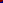
\includegraphics[width=5mm]{shapes/15.png} & 1.\\
        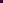
\includegraphics[width=5mm]{shapes/11.png} & 2.\\
    \end{tabular}
    \caption{Weights for selected shapes.}
    \label{table:shapes}
\end{table}

This choice of prior is similar to the Ising model. In the Ising model, all
cliques are pairs of neighbors. This structure is able to assert that neighbors
should mostly be the same label. However, it is not able to assert the likely
boundaries between two segments. Our generalization hopes to assert likely
boundaries along with the core idea that neighbors should mostly be the same
label.

discuss motivations for choosing special clique configurations. 

discuss how this is an attempt to generalize or improve upon Ising model, where
only adjacent pixels are considered.

discuss the Gaussian model for pixel emission, as well as the choice for conjugate priors.(abe)

\subsection*{Results}(Matthew)
Stick in images, discuss parameters used such as segments, factor weights.
Show plots of Gibbs sampler convergence.


\subsection*{Qualitative Evaluation}
We hope that the decisions made about the prior structure of the segments will
help the model be less sensitive to pixel anomalies that might be present if
the labels were treated as independent. For example, if a single was a
different color than most of its neighbors, the prior influence would hopefully
be such that this anomaly would be ``squeezed out'', and it would be labelled
with its neighbors.

There is a trade-off between the size of the cliques and the complexity of their
implementation and computation. Since we are not learning the factor weights,
but rather specifying them ``by hand'', more complex cliques would result in
more time spent making decisions about which shapes to assert or penalize.
Also, every clique of which an individual label is a member needs to be
including in the Gibbs sampling update. So the computational complexity
increasing with the complexity of the cliques.

Since we choose to work with small, simple cliques, their influence is mostly
seen at the local level. They are able to help influence the micro-structures
that are exhibited among the segments. However, they do not have a macroscopic
view of the problem. This can result in fragmented segments.

RGB space different from human qualitative perception, which affects cluster assignments.
Is there an ideal color space corresponding to human perception? (Abe)

Model doesn't account for texture, just assumes each cluster is largely one color (or point 
in RGB space). (Abe)


\subsection*{Conclusion} (Matthew)
This model presents interesting ideas about image segmentation, and also
demonstrates important shortcomings. The structure for the prior distribution
of segments allows an interesting paradigm in which to work. However, there are
certain deficiencies that necessarily arise when working on a local scale.

One important decision we made as modelers was to use a generative model. This
gave us an intuitive way to approach the problem. However, we feel like it
would be worthwhile to explore using conditional models for this problem.
Generating new images with the model does not have many apparently practical
purposes. Using a generative model would allow the distribution on a label to
involve not only the pixel emission it labels, but also the emissions of its
neighbors or others. This would allow another mechanism to help detect
boundaries.

By completing this project, we learned a lot about specifying and working with
hybrid directed-undirected graphical models. Also, we developed our intuition
about what important questions need to be answered when segmenting an image.
Finally, we developed our modeling abilities by creating and working with a new
probability model.
\end{document}
